%==============================================================================%
\chapter{Applications and Visualisations} \label{chapter:applications}
%==============================================================================%
This chapter serves as a gallery of possible applications that can arise from the data generated from the Smart Street Sensor project. 
As was  seen in Chapter \ref{chapter:literature}, availability of granular, longitudinal data on the movement and distribution of people at such spatial extent has numerous uses in various fields of study. 
This chapter first starts by looking at the use of the data in understanding the broad footfall landscape of the United Kingdom (UK), deriving sample insights on how retail footfall in the UK has been performing for the past couple of years along with some sample analysis from the national level to individual locations to understand the nature and change of footfall.
It then demonstrates couple of ways of detecting events and their effect on places from the change in the footfall volumes.
Finally the chapter briefly describes a way to calculate the flow of pedestrians between the locations just from the highly granular footfall volume using a probabilistic approach.

%------------------------------------------------------------------------------%
\section{United Kingdom Footfall Index}
%------------------------------------------------------------------------------%
One of the broad questions that arises when such footfall data is available is about the general national trend of footfall on retail high streets.
This national 'footfall index' is not only important for the retail industry but also for various other purposes such as policy making, economic forecasting, etc.
Since the footfall has a weekly periodicity, a standardised index could be arrived from sensor based data by aggregate them at a national level and find the average footfall at every location at every week. 
Although this is a simplistic measure, it does a good job in describing the changes in the retail footfall in the UK as a whole.
From the last two years, it can be observed that retail footfall in UK started at its lowest in the beginning of the year and increased steadily until spring.
The high footfall lasted through the summer months before going down steadily towards the end of the year..
This trend changed around the fall months and the footfall reached the highest in the first two weeks of December and fell back to the lowest in the last two weeks.
This form the yearly pattern of retail footfall in UK is illustrated in Figure \ref{figure:applications:footfall:index} which shows the weekly footfall index of the UK from 2017 to 2018. 

\begin{figure*}
  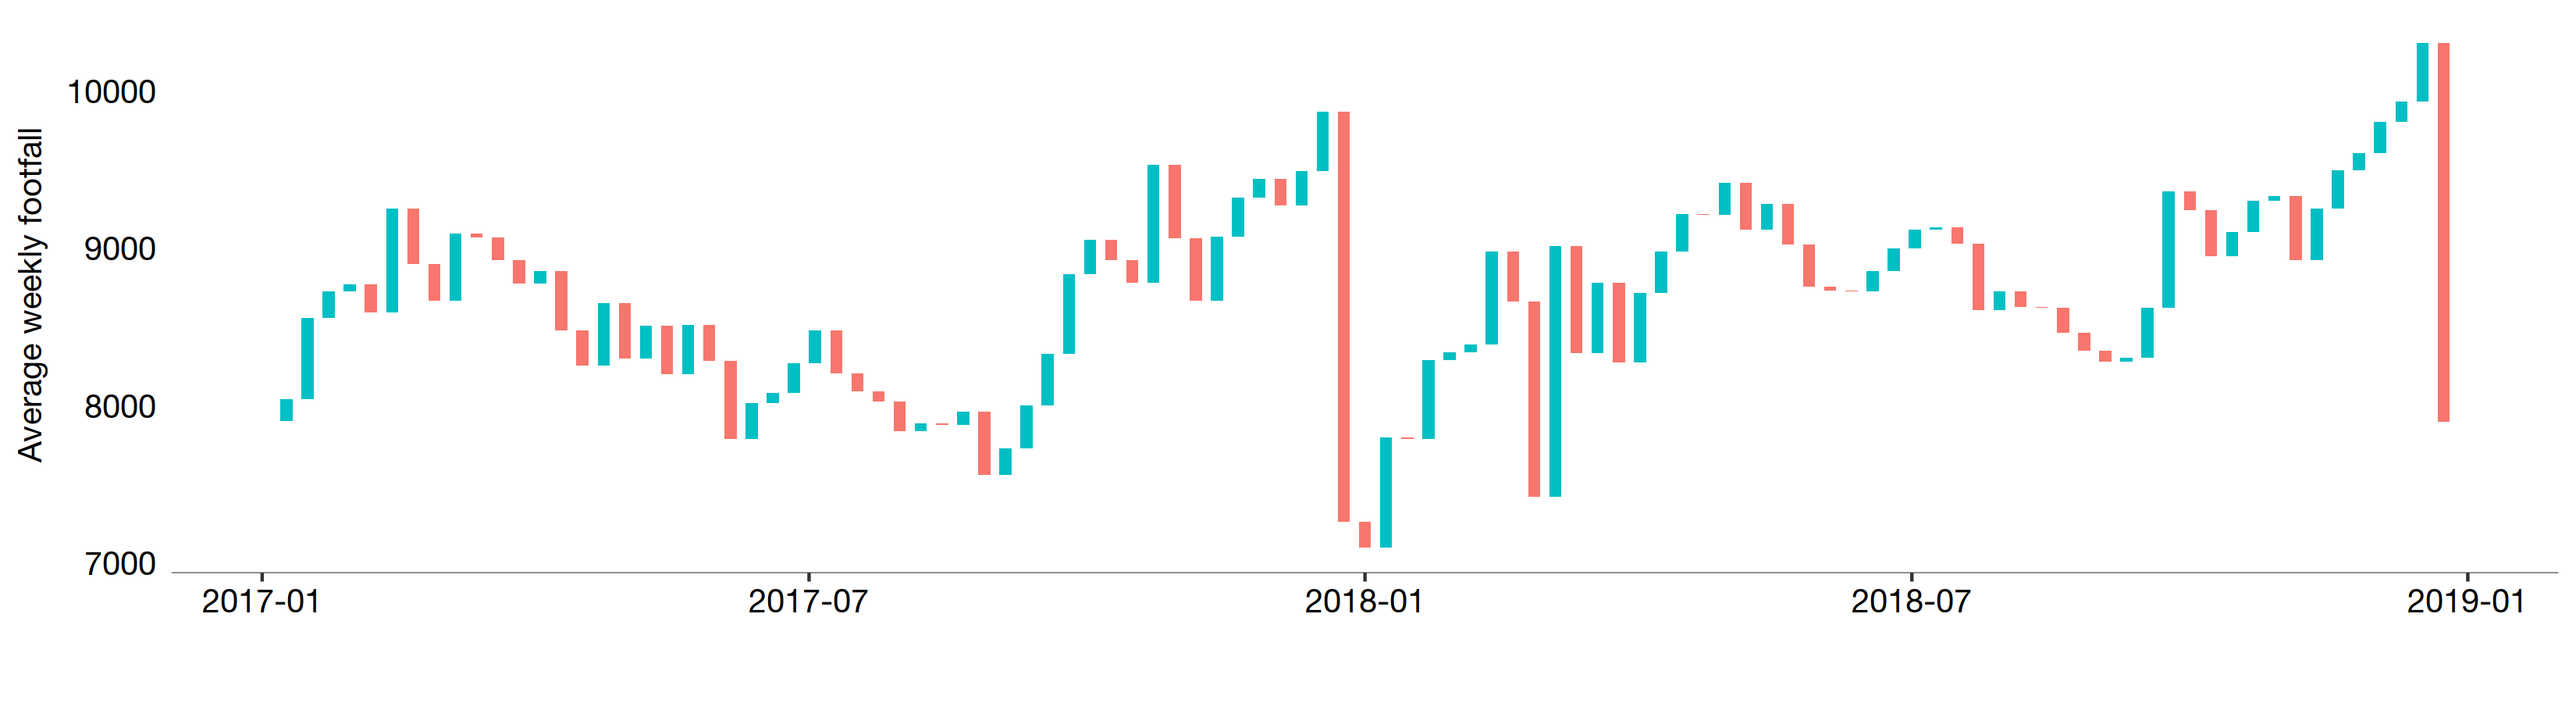
\includegraphics[trim={0 25 0 10},clip]{images/applications-footfall-index.png}
  \caption{A weekly footfall index for United Kingdom showing the change in footfall from 2017 to 18}
  \label{figure:applications:footfall:index}
\end{figure*}

In addition to showing larger trends, this footfall index also showed sudden short term changes. 
One such as example was the storm in February 2018 which corresponded with some of the lowest footfall experience across the UK.
This `footfall index' can serve as a measure to give the overall outlook for the 
retail activity in the country at any given week.

\subsection{City-wise footfall index}

Being derived from location-wise data, the index could be calculated for geographic extents as well.
For example, Figure \ref{figure:applications:cities:change} shows the spatial distribution of footfall change in the UK towns between 2017 and 2018.
On a glance, it can be observed that the small southern towns such Ipswich, Staines, Southend by Sea and Plymouth had a good amount of growth in footfall while the towns such as West Bromwich, Derby and Warrington have a decline in footfall.
In addition to long term changes, from the footfall data, even insights on short term changes could be derived.
For example, Figure \ref{figure:applications:cities:month} shows the change in footfall from the previous year for towns across UK for just the months of April and May 2019.
It can be observed that April 2019 has been slower than last year in most towns across UK while May 2019 has been actually better than last year.
This kind of granular insights into trends in footfall could be valuable for local authorities who can measure and monitor the health of their retail areas closely.

The difference in even smaller intra-day patterns in cities could be derived from footfall data which could show the nature of their economies
Figure \ref{figure:applications:cities:profiles} shows an average daily footfall pattern for 9 cities in the UK.

\subsection{Location profiles}
One of the most interesting insights that can be derived from the dataset is the detailed knowledge of the locations themselves.
The data can not only reveal how popular a location is but also the exact times when the location is popular.
The patterns in the usage of the locations could also reveal the function of the place giving us the opportunity to measure their change through time as well.
For example, Figure \ref{figure:applications:location:profiles} shows the daily footfall profile of three locations in London for two weeks in 2019.
It can be observed that all three locations have completely different patterns of usage.
Leicester Square was mostly a night time destination where the footfall peaks around evening while Regent street is a mostly office location with three distinct peaks corresponding to morning commute, evening commute and lunch.
These insights can be crucial for retailers operating in these places for optimising their business operation in terms of store opening times, scheduling shifts etc.

\begin{figure*}
  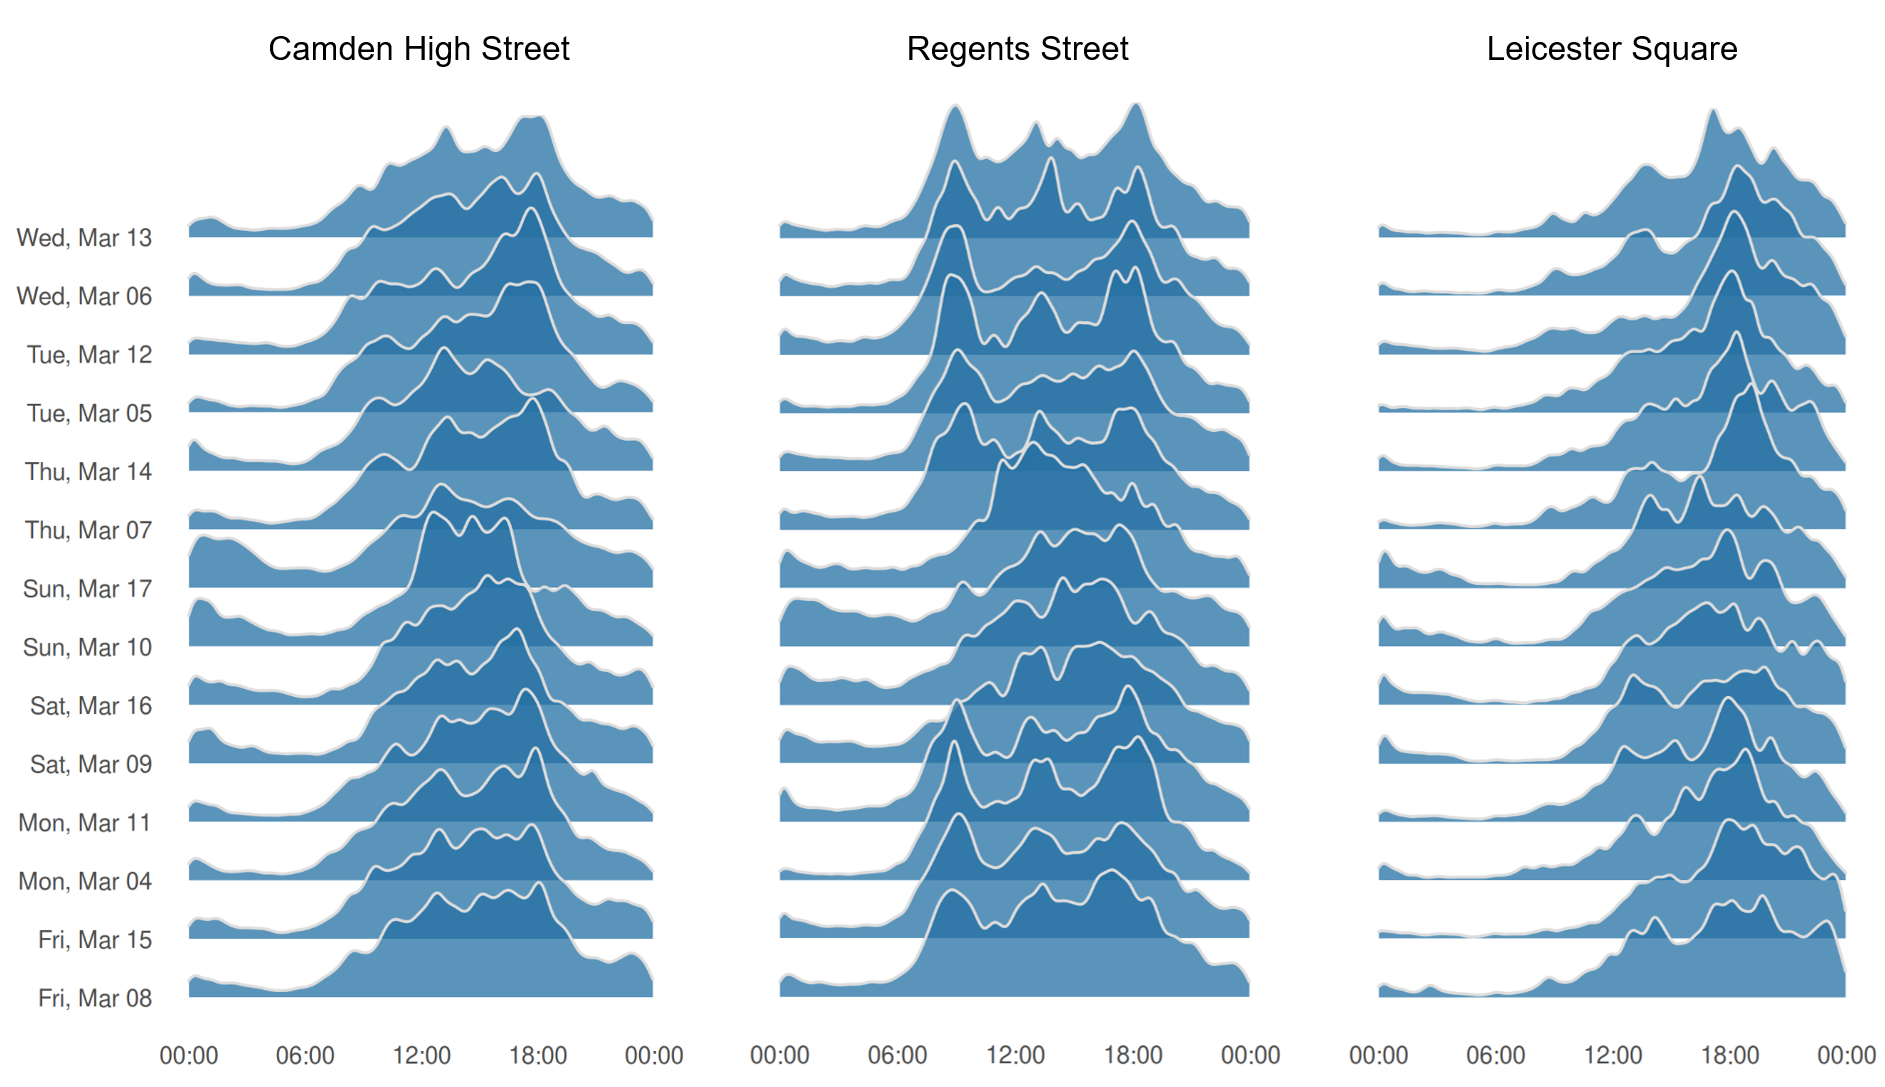
\includegraphics[trim={0 10 0 0},clip]{images/applications-location-profiles.png}
  \caption{The profiles can be tracked longitudinally to reveal nature and change.}
  \label{figure:applications:location:profiles}
\end{figure*}

Another way to understand the evolution of a place over time is to look at the patterns of its usage over the corresponding period.
For example, Figure \ref{figure:applications:footfall:calendar} shows a 'footfall calendar' for Old street, London which traces and visualises the evolution of the place for the first half of 2018.

%------------------------------------------------------------------------------%

\cleartoleftpage
\begin{figure*}
  \forceversofloat
  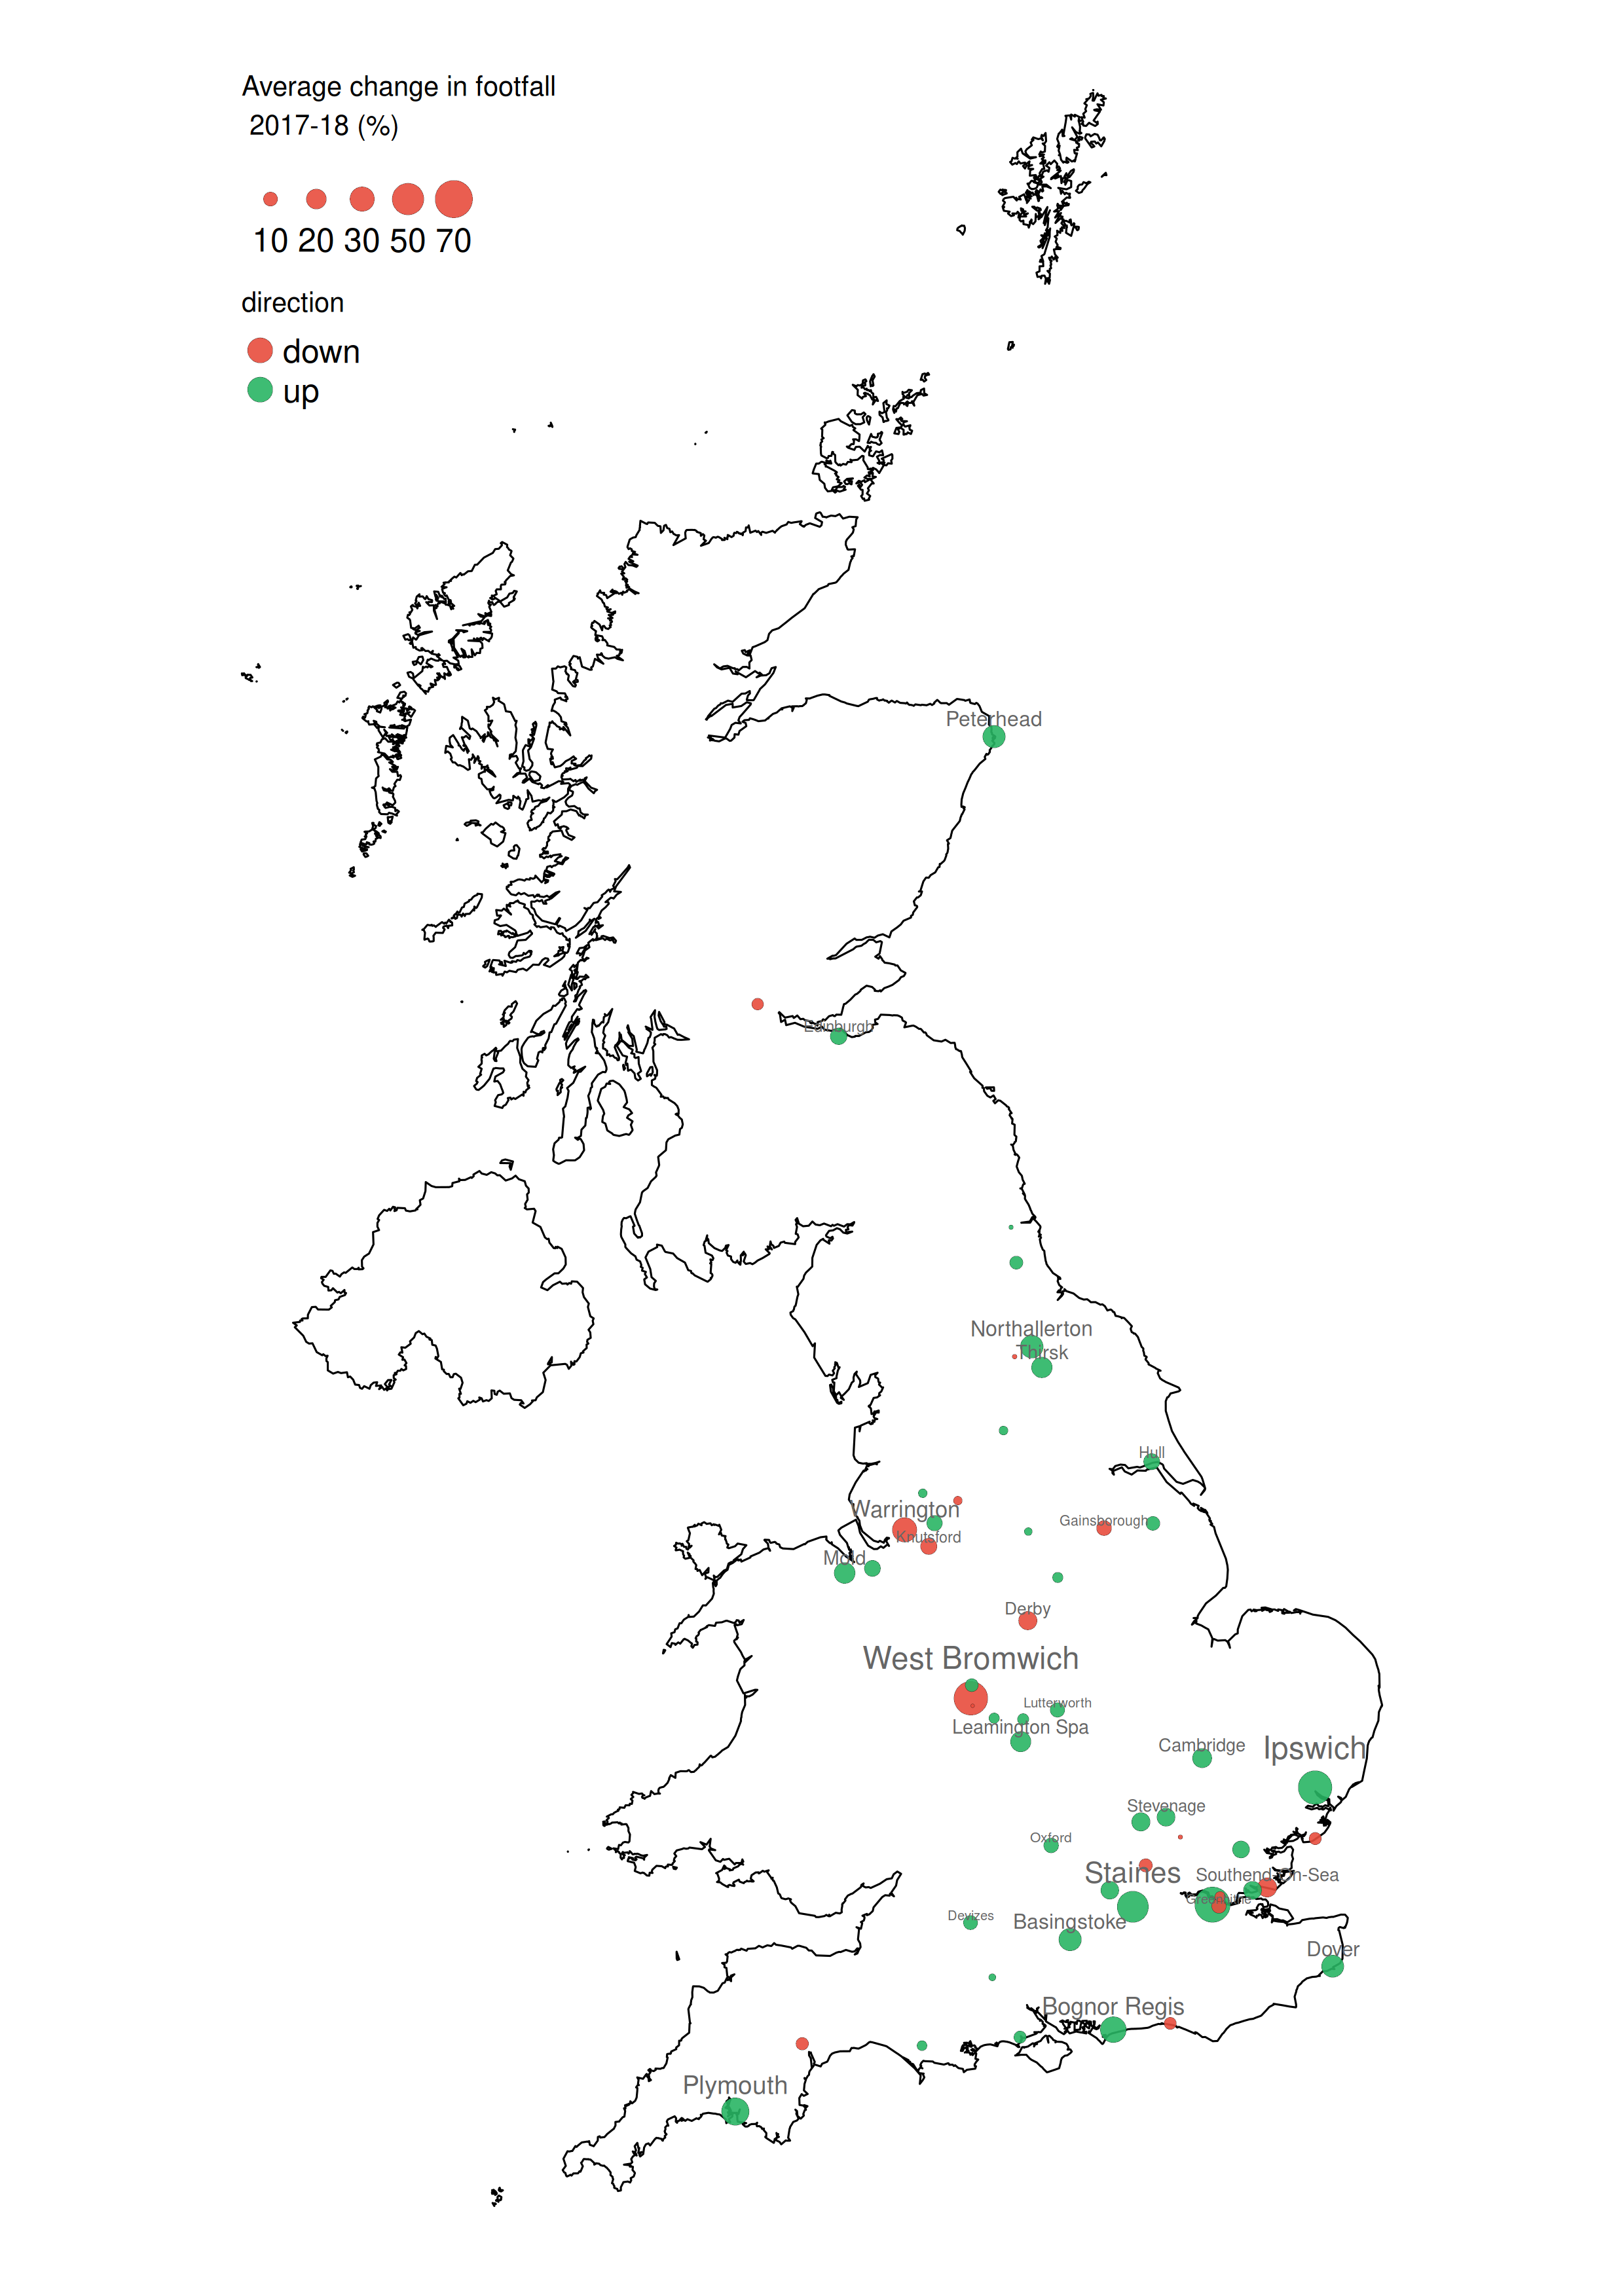
\includegraphics[trim={0 0 0 0},clip]{images/applications-cities-rank.png}
  \caption{The change (\%) in average weekly footfall of towns across the UK in 2018 compared to 2017.}
  \label{figure:applications:cities:change}
\end{figure*}

\begin{figure*}
  \forcerectofloat
  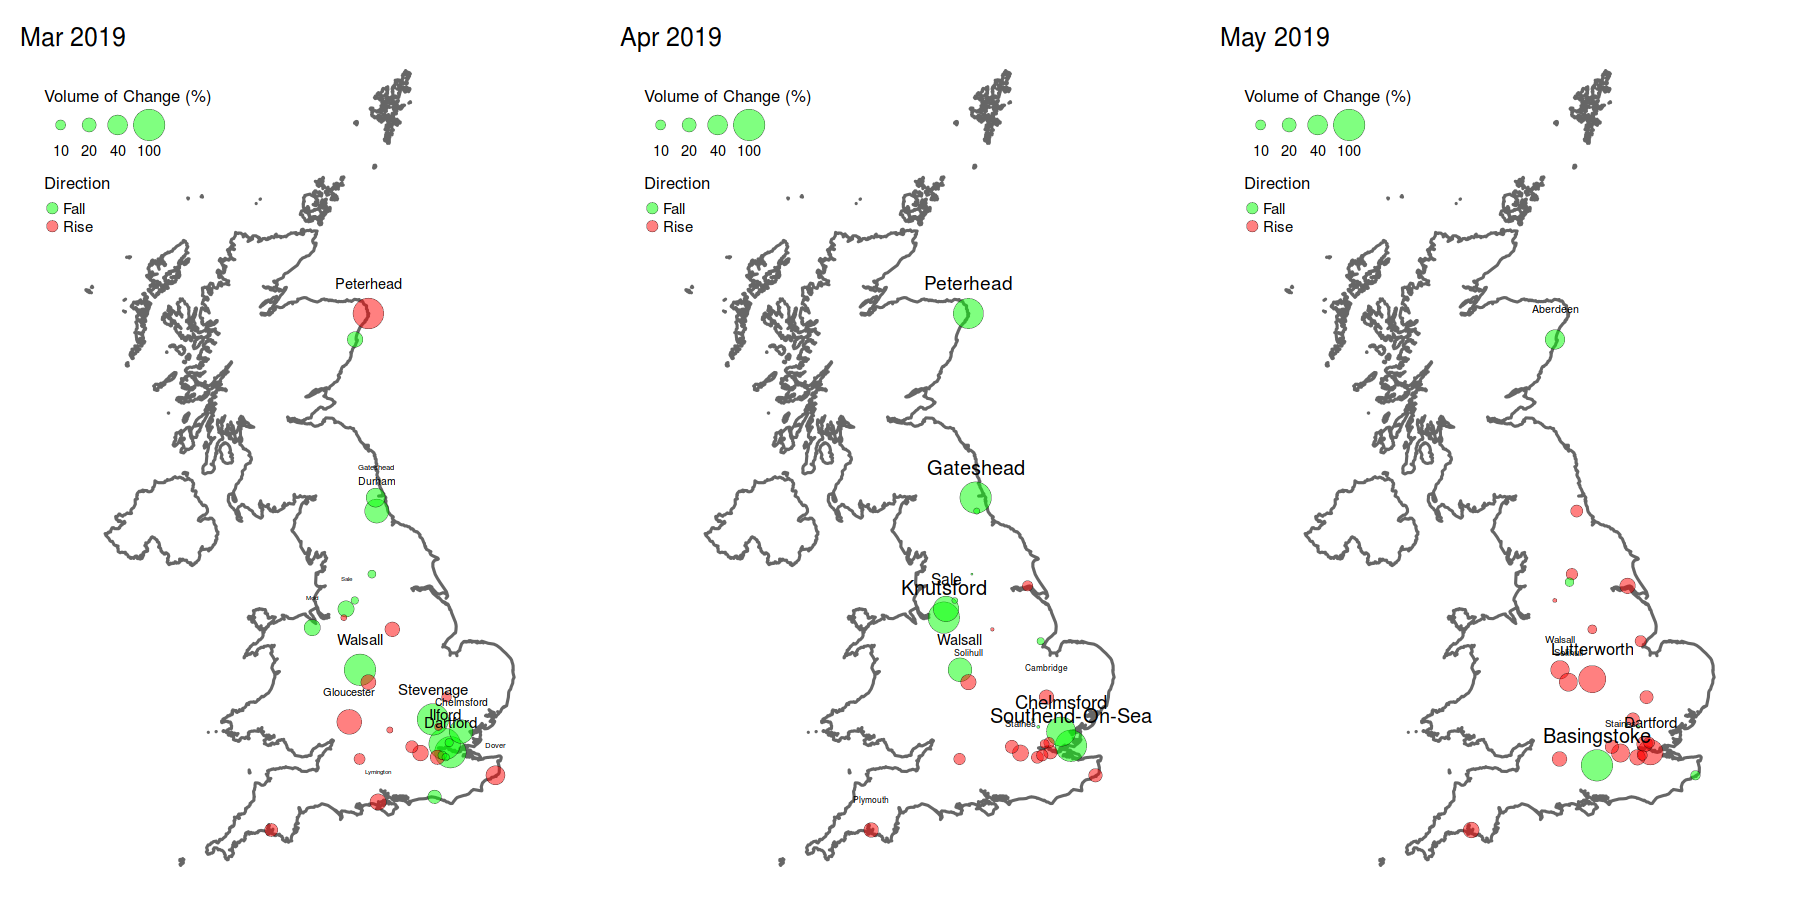
\includegraphics[trim={0 12 0 0},clip]{images/applications-city-indices.png}
  \caption{The change (\%) in monthly average footfall in towns across the UK in April and May 2009.}
  \label{figure:applications:cities:month}
\end{figure*}

\begin{figure*}
  \forcerectofloat
  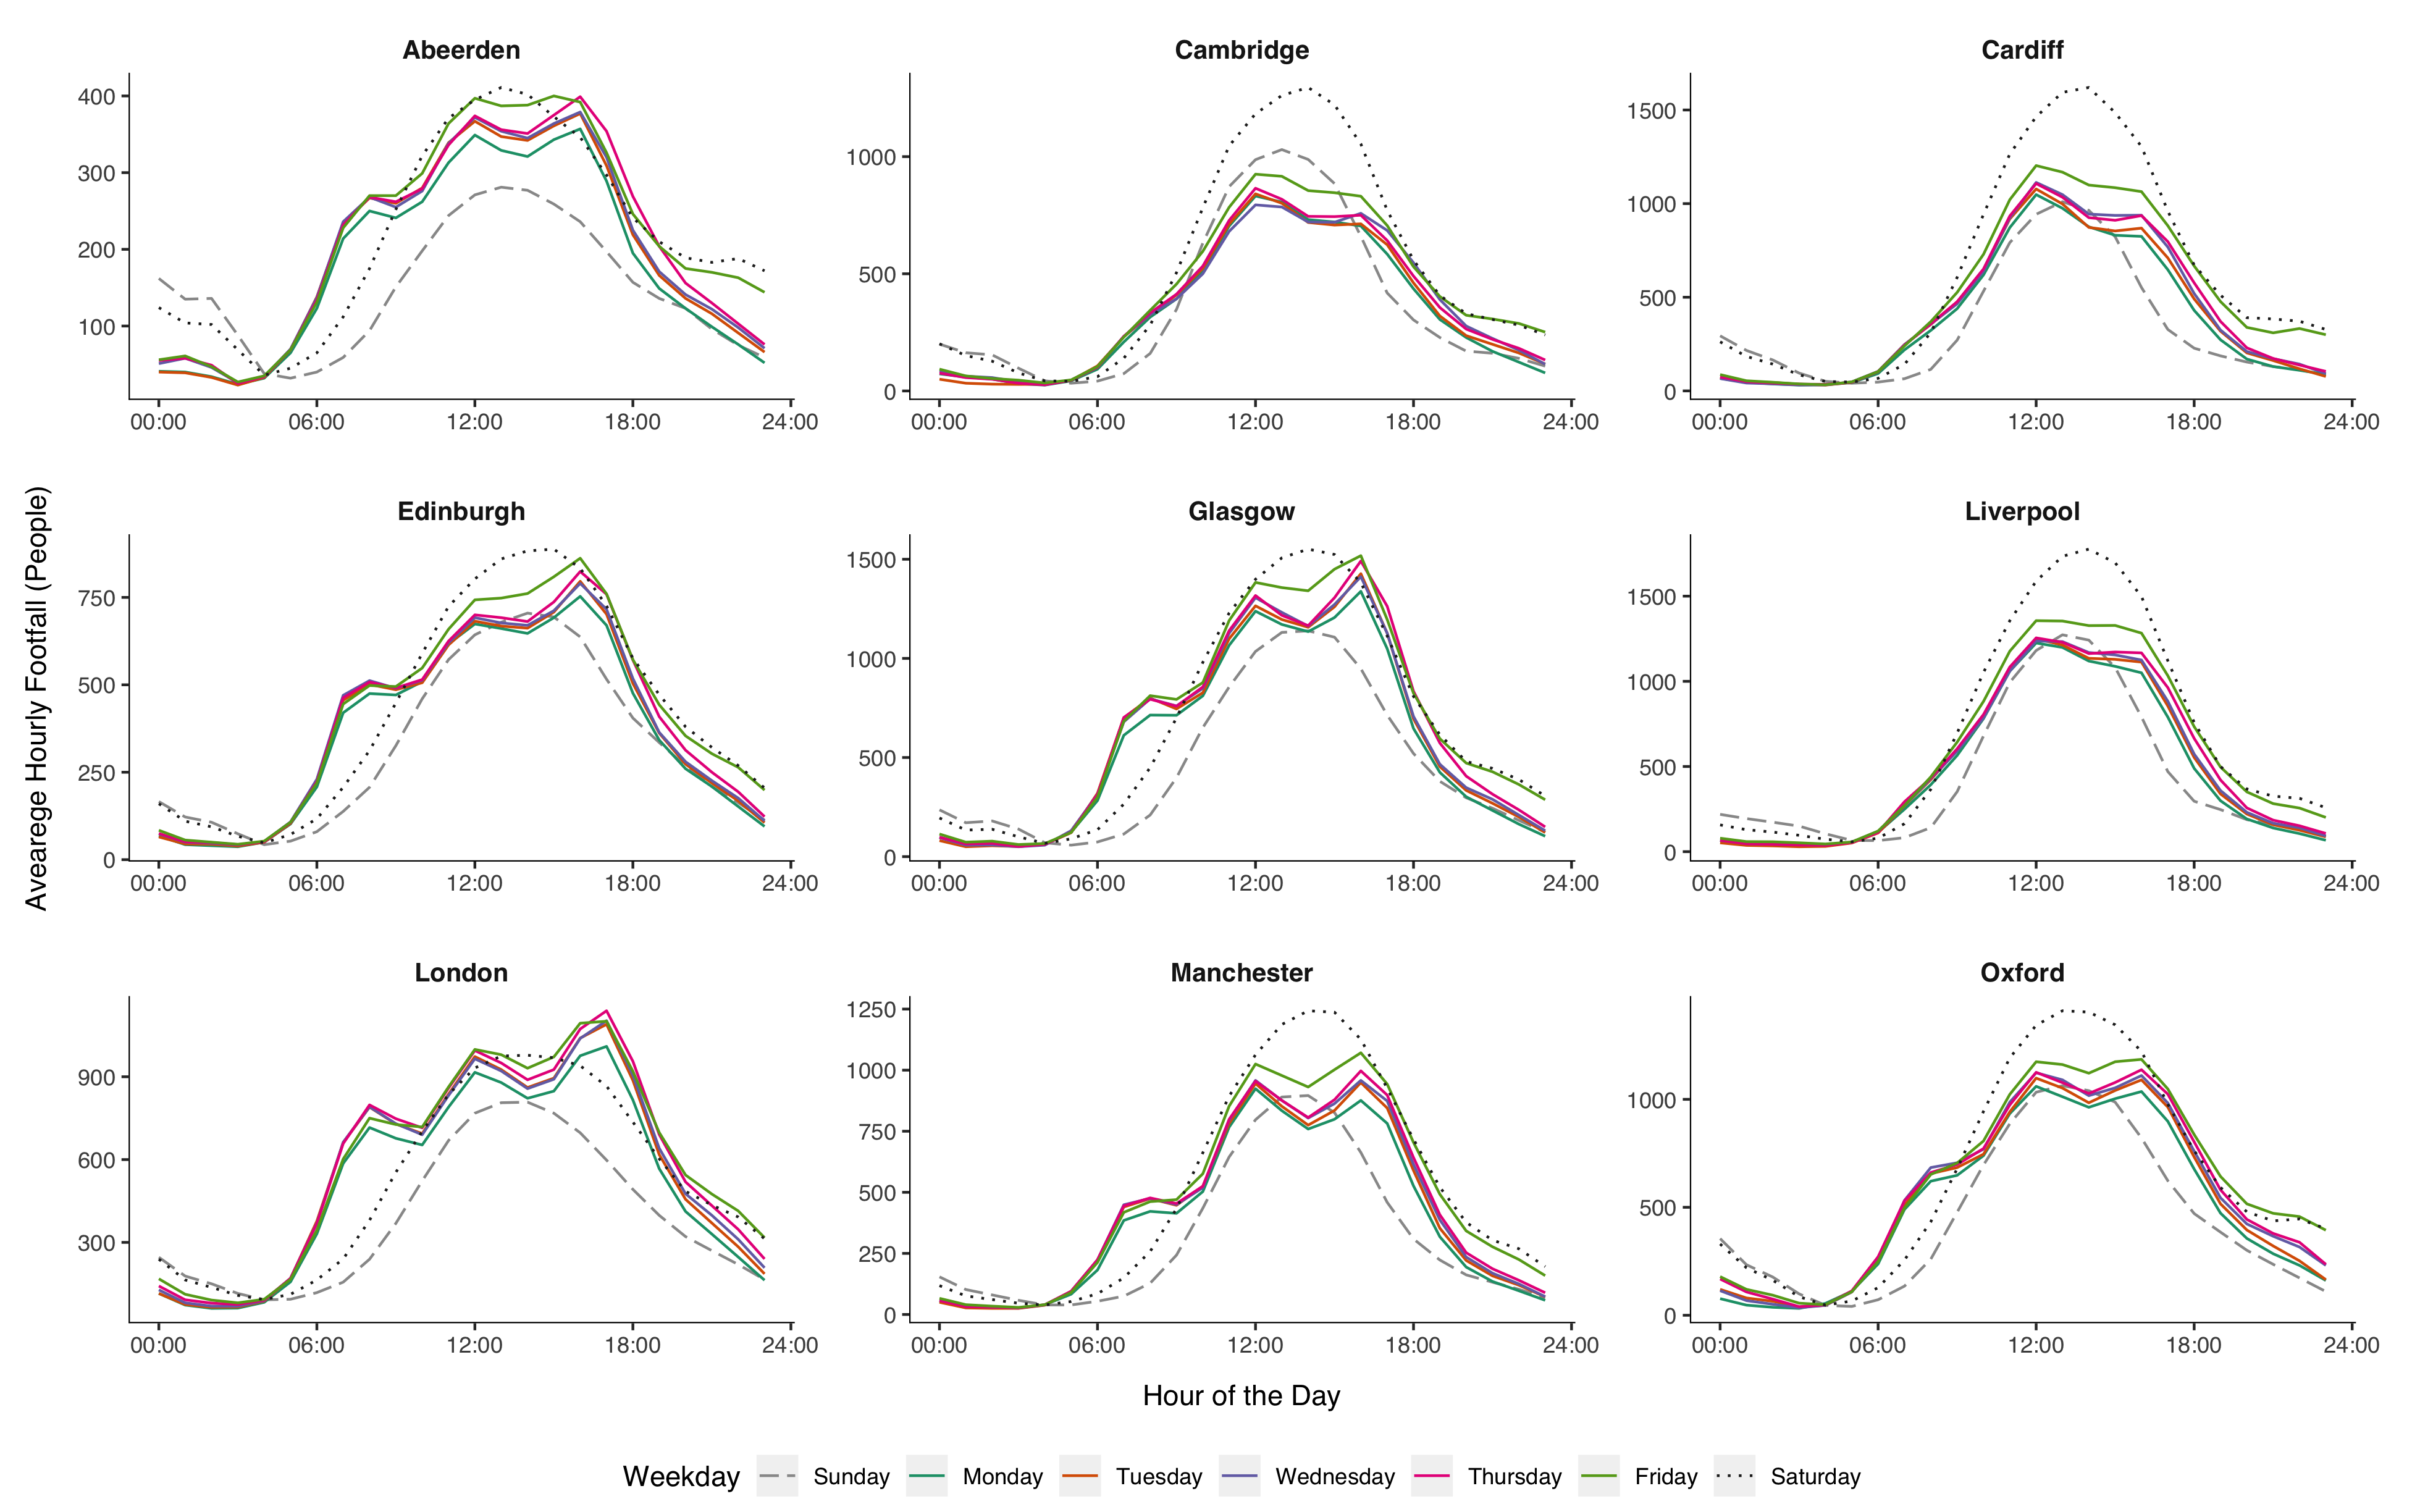
\includegraphics[trim={0 10 0 0},clip]{images/applications-city-profiles.png}
  \caption{Intra-day footfall profile of major cities in United Kingdom}
  \label{figure:applications:cities:profiles}
\end{figure*}

%------------------------------------------------------------------------------%
\cleartoleftpage
\newgeometry{
  left=20mm,
  textwidth=122mm,
  marginparsep=7mm,
  marginparwidth=43mm
}
\begin{figure*}
  \forceversofloat
  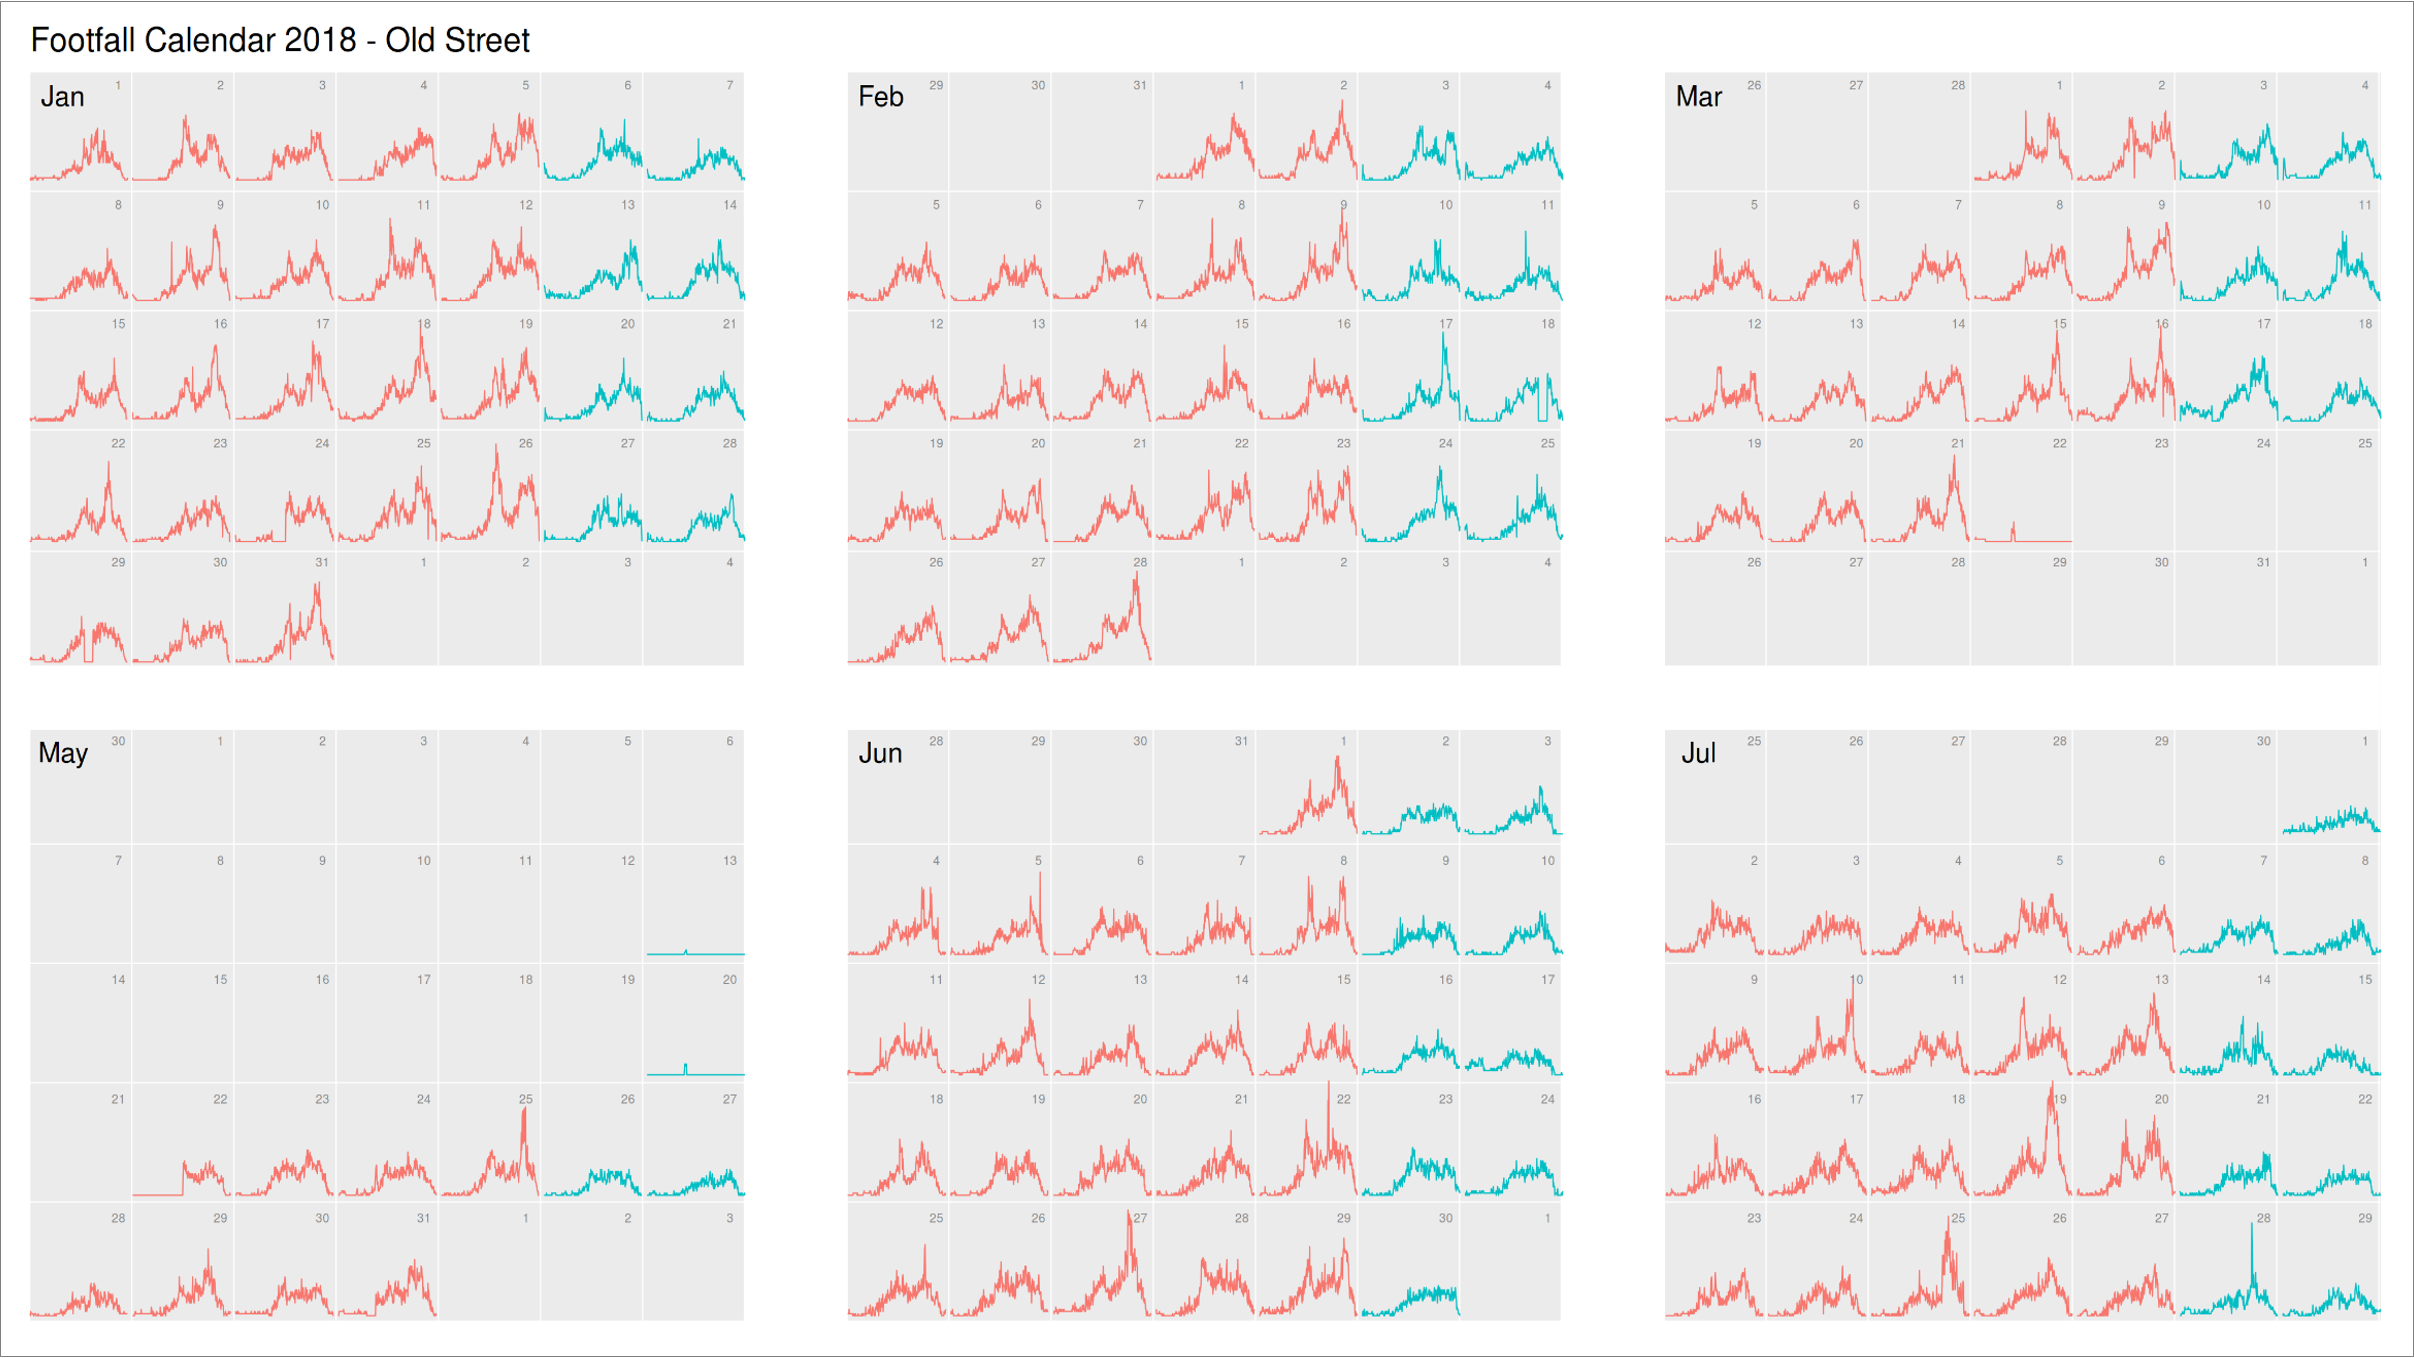
\includegraphics[width=172mm,trim={0 0 1310 -42},clip]{images/applications-footfall-calendar.png}
  \caption{Footfall calendar showing the profiles of daily volumes of footfall at Old Street, London.}
  \label{figure:applications:footfall:calendar}
\end{figure*}
\clearpage
\begin{figure*}
  \forcerectofloat
  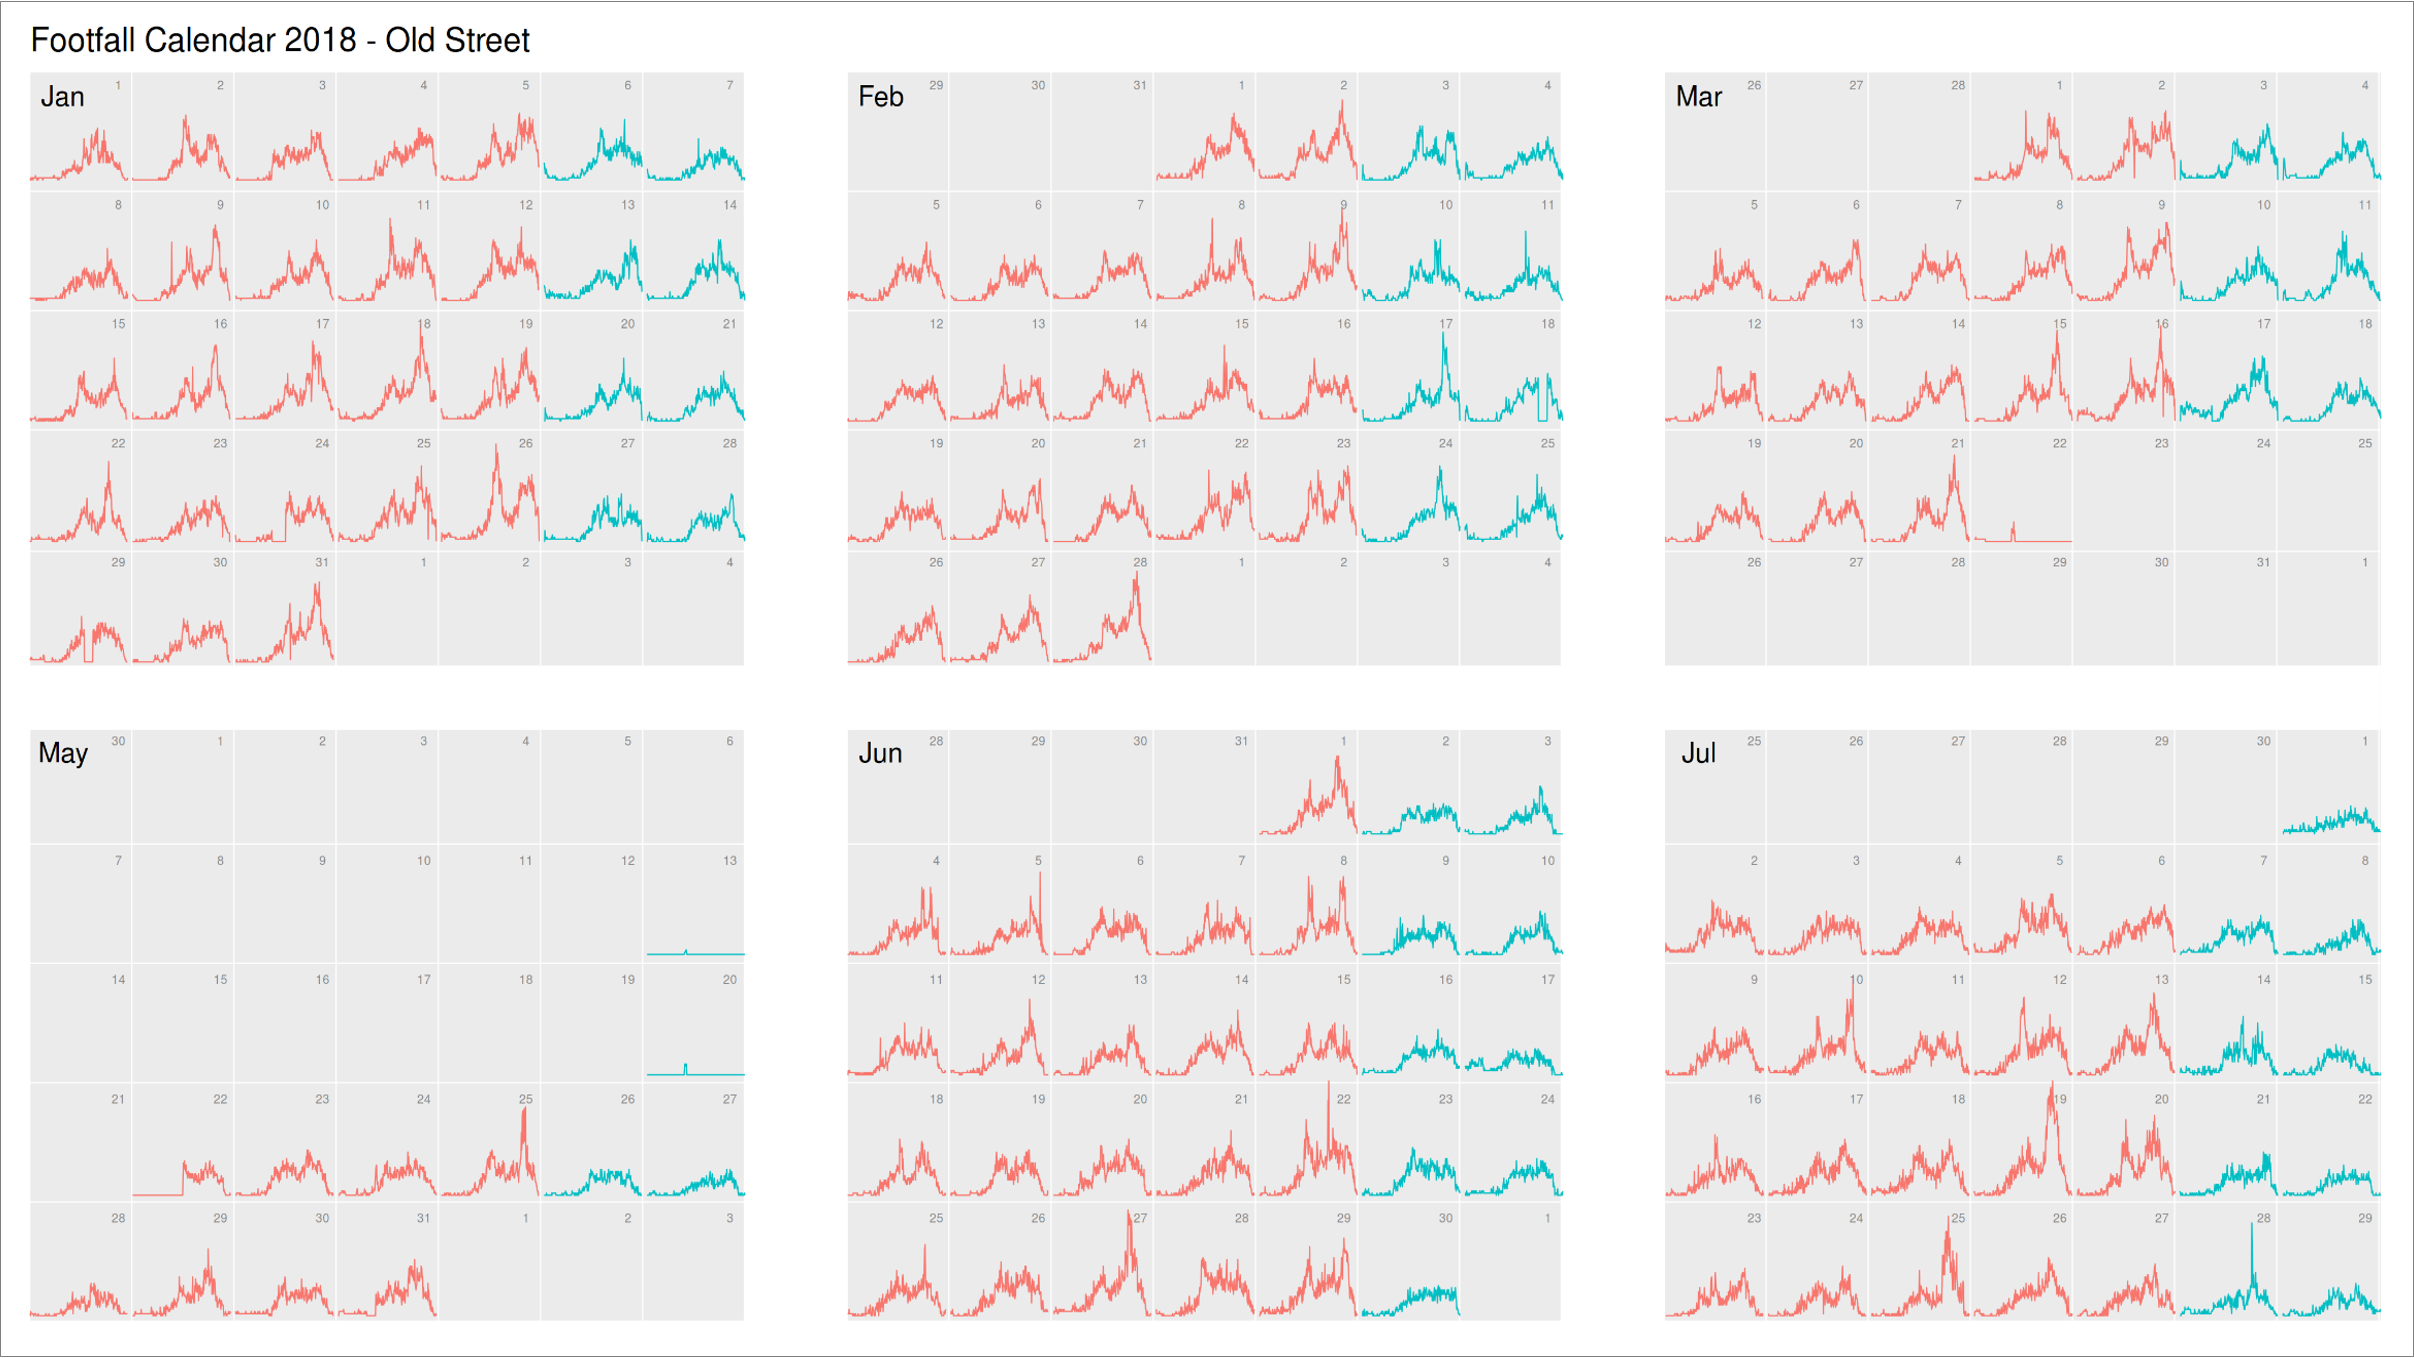
\includegraphics[width=172mm,trim={1315 0 0 0},clip]{images/applications-footfall-calendar.png}
  \caption[]{}
  \label{}
\end{figure*}
\restoregeometry
\clearpage

%------------------------------------------------------------------------------%
\section{Event Detection}
%------------------------------------------------------------------------------%

When footfall is looked at longitudinally across locations, a wide range of information can be uncovered about the context which resulted in the patterns in the footfall. 
Figure \ref{figure:applications:cardiff} shows the normalised weekly footfall of 10 different locations across Cardiff for two years: 2017 and 2018. 
The patterns in the footfall clearly show numerous events that were happening in Cardiff as unusually high or low footfall in the corresponding week. 
The most significant event was in February 2018, when all sensors reported the lowest numbers they have ever recorded. 
This coincided with the cold wave in UK named ‘Beast from the East’, which brought adverse weather conditions all over the UK and led to a significant reduction in footfall. 
The other identifiable events are bank holiday weekends which result in higher than normal footfall, and the holiday shopping season when footfall is at its highest. 
Finally, it is interesting to see the difference in summertime footfall between 2017 and 2018, which could be explained by the FIFA World Cup which took place in the summer of 2018. 
This example shows the usefulness of the footfall data to detect real life events from the data in near real time. 
It can also be used to measure the effect of events on footfall, and hence understand the impact of these events for retail and the  economy more generally.

\begin{figure*}
  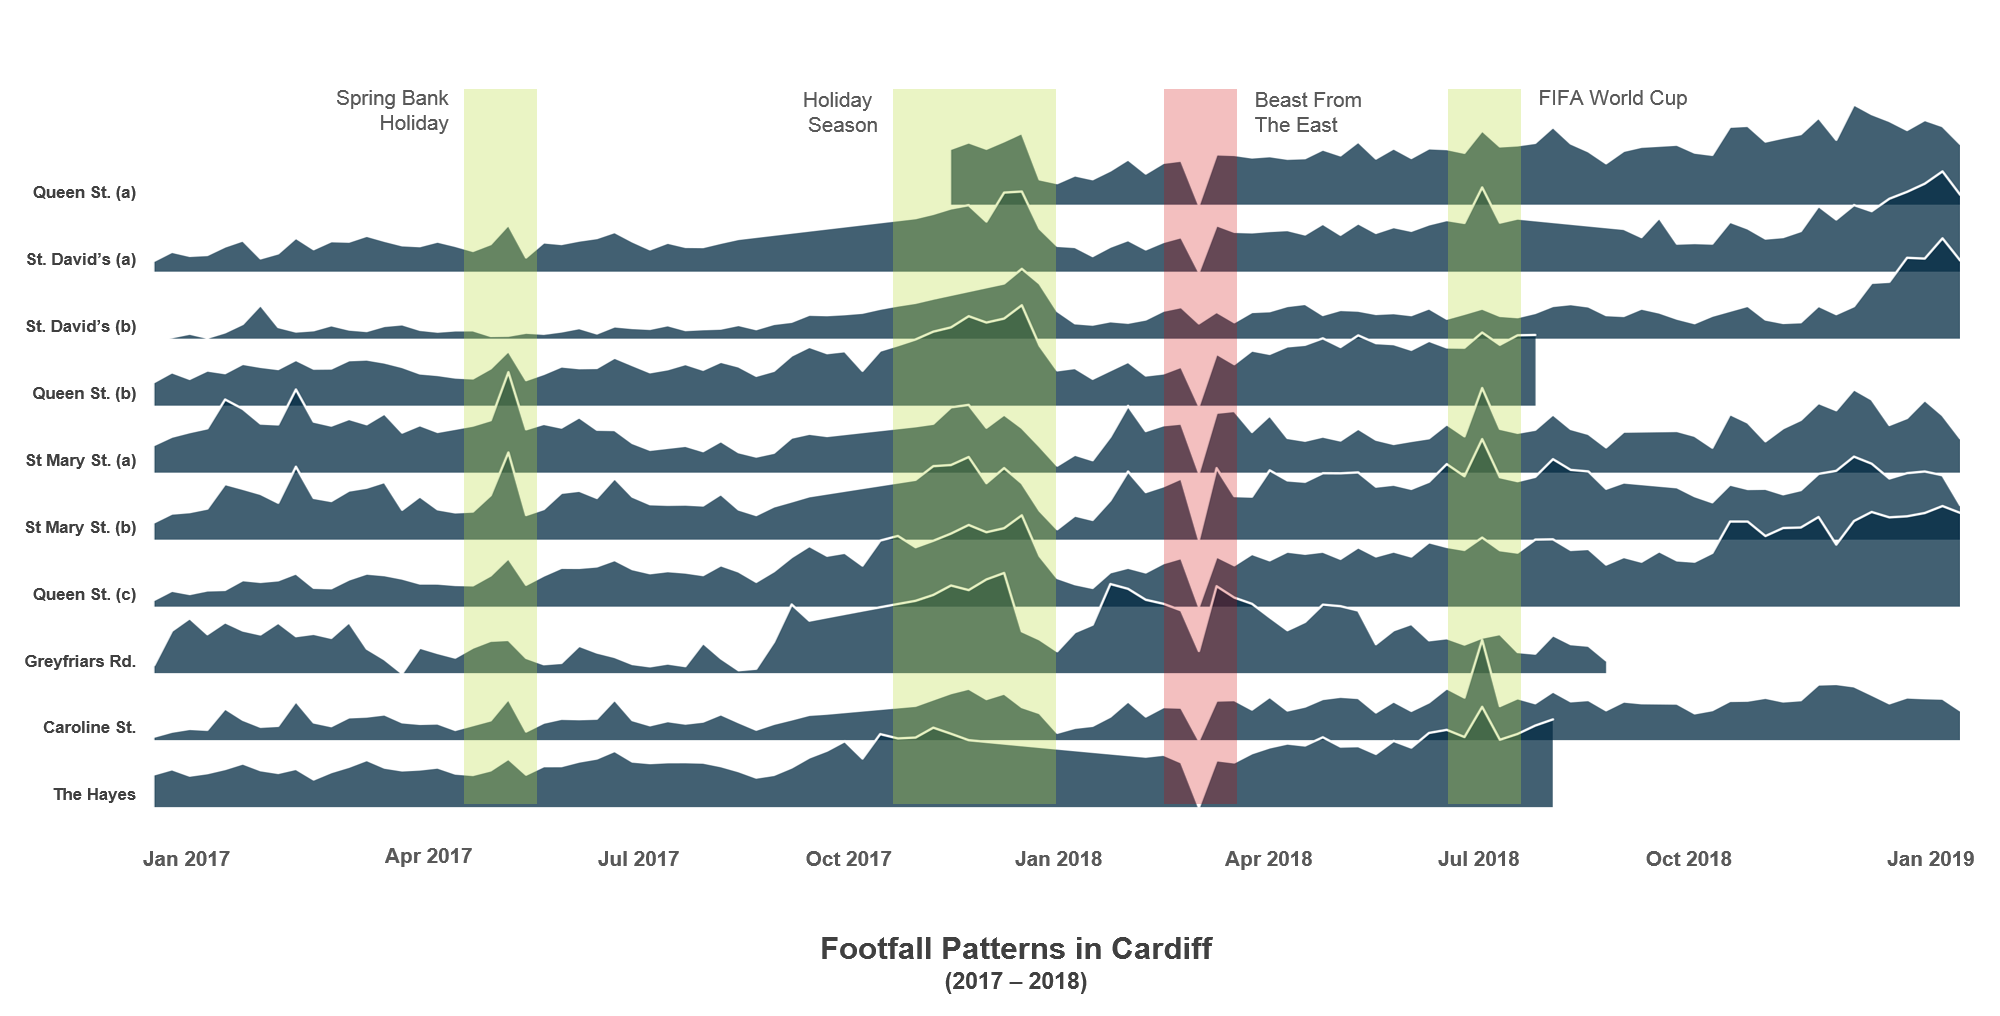
\includegraphics[trim={0 50 0 0},clip]{images/applications-cardiff-footfall.png}
  \caption{Normalised weekly footfall index at locations across Cardiff from 2017 to 2018}
  \label{figure:applications:cardiff}
\end{figure*}

\subsection{Football world cup}
In addition to long-term changes and events, the footfall data can be used to identify the smaller effects of these events at an area scale.
Figure \ref{figure:applications:football} shows footfall from two days in Leicester square, London when the quarterfinal and semifinal matches of the 2018 FIFA World Cup took place. 
Both matches happened in the evening and led to an  increase in footfall around match time. 
The most interesting observation is the effect the outcome of the game had on footfall. 
On the day of the quarterfinal, the winning result of the English team led to a post-match celebration which pushed the Leicester Square footfall to its day-time highest, unlike the day of the semifinal when the English team lost. 
This not only shows the usefulness of the data in understanding the effect events have on local footfall, but it also shows how the data can be used by retailers to predict the effect the results of sports events might have on them.

\begin{figure}
  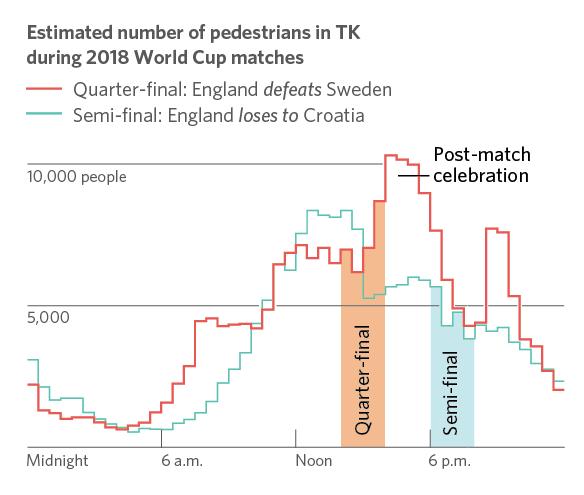
\includegraphics[trim={0 0 0 0},clip]{images/applications-football-sample.png}
  \caption{The difference in footfall distribution at Leicester square, London after the FIFA World Cup quarterfinal and semifinal matches. Source: Oliver Uberti and James Cheshire }
  \label{figure:applications:football}
\end{figure}

These examples show the importance of footfall data in detecting events. 
Even a simple visual analytics of the dataset reveal interesting information on events. 
This would be much more useful when used in tandem with advanced machine learning/data mining techniques, and will predict much better results as more data is collected.

%------------------------------------------------------------------------------%
\section{Pedestrian Flows}
%------------------------------------------------------------------------------%

Detecting general trends in the flow of people between spatial locations is neither obvious nor a trivial task. 
This is due the high cost of capturing these movements without compromising people’s privacy, since the primary way to collect such detailed data involves handling people’s precise location data. 
This research specifically removes any personally identifiable information because of MAC randomisation and hashing, and therefore seems like it might not be suitable for studies on human mobility. 
However, this problem can be solved by examining the movement of people in the Smart Street Sensors network at a fine spatial and temporal resolution using a novel methodology in the field of Big Data which uses mathematical models from information theory: Transfer Entropy (TE). 
Using an area in central London, this section serves as a case study to demonstrate the usefulness of TE as a measure of the flow of pedestrians\sidenote{Work undertaken was in collaboration with Roberto Murcio and Karlo Lugomer. 
The methodology was formulated by Murcio; this author worked on the implementation of the method in the case study.}.

Consider the array of sensors shown in Figure \ref{figure:applications:transent} and assume that there is a flow of people walking past Location 116 and then diffusing towards the remaining sensors. 
Counts generated by the sensor are aggregated per five minute intervals, so if, for example, it takes one minute to walk from Location 116 to Location 117, the number of people detected at 117 from minutes 2 to 5, would correspond to the percentage of people detected at 116 from minutes 1 to 4. 
In other words, the similarity between the time series of counts at the locations under consideration are correlated. 
Hence the aim here is to provide a measure for the size of the flow between each pair of sensors without actually tracking individual people. 
One way to accomplish this, is to think of this motion of people as flows of information among distinctive sources, so we can relate the number of people reaching one sensor from another by measuring the uncertainty between two interacting random variables. 
For this, we used an information theory concept known as Transfer Entropy (TE) defined by:

\begin{equation} \label{equation:te}
  TE(X,Y) = \sum_{t=1} p(y_{t+1}, y_{t}, x_{t}) \times { log{ \frac{p(y_{t+1} \mid y_{t}, x_{t})}{p(y_{t+1} \mid y_{t})}} }
\end{equation}

Where $t$ indicates a given point in time.
Equation \ref{equation:te} measures the reduction in uncertainty at $y_{t}$, given $x_{t}$ and $y_{t-1}$.
In comparison with the case when only $y_{t-1}$ is known.
This measure is applied directly to our people's movement problem and $X$ = location i, $Y$ = location j and $t$ runs for a whole day, the $TE$ would represent an indicator for the direction of the flow, as the counts at $y_{t+1}$ are more accurately estimated using the information of $x_{t}$.

\begin{figure*}
  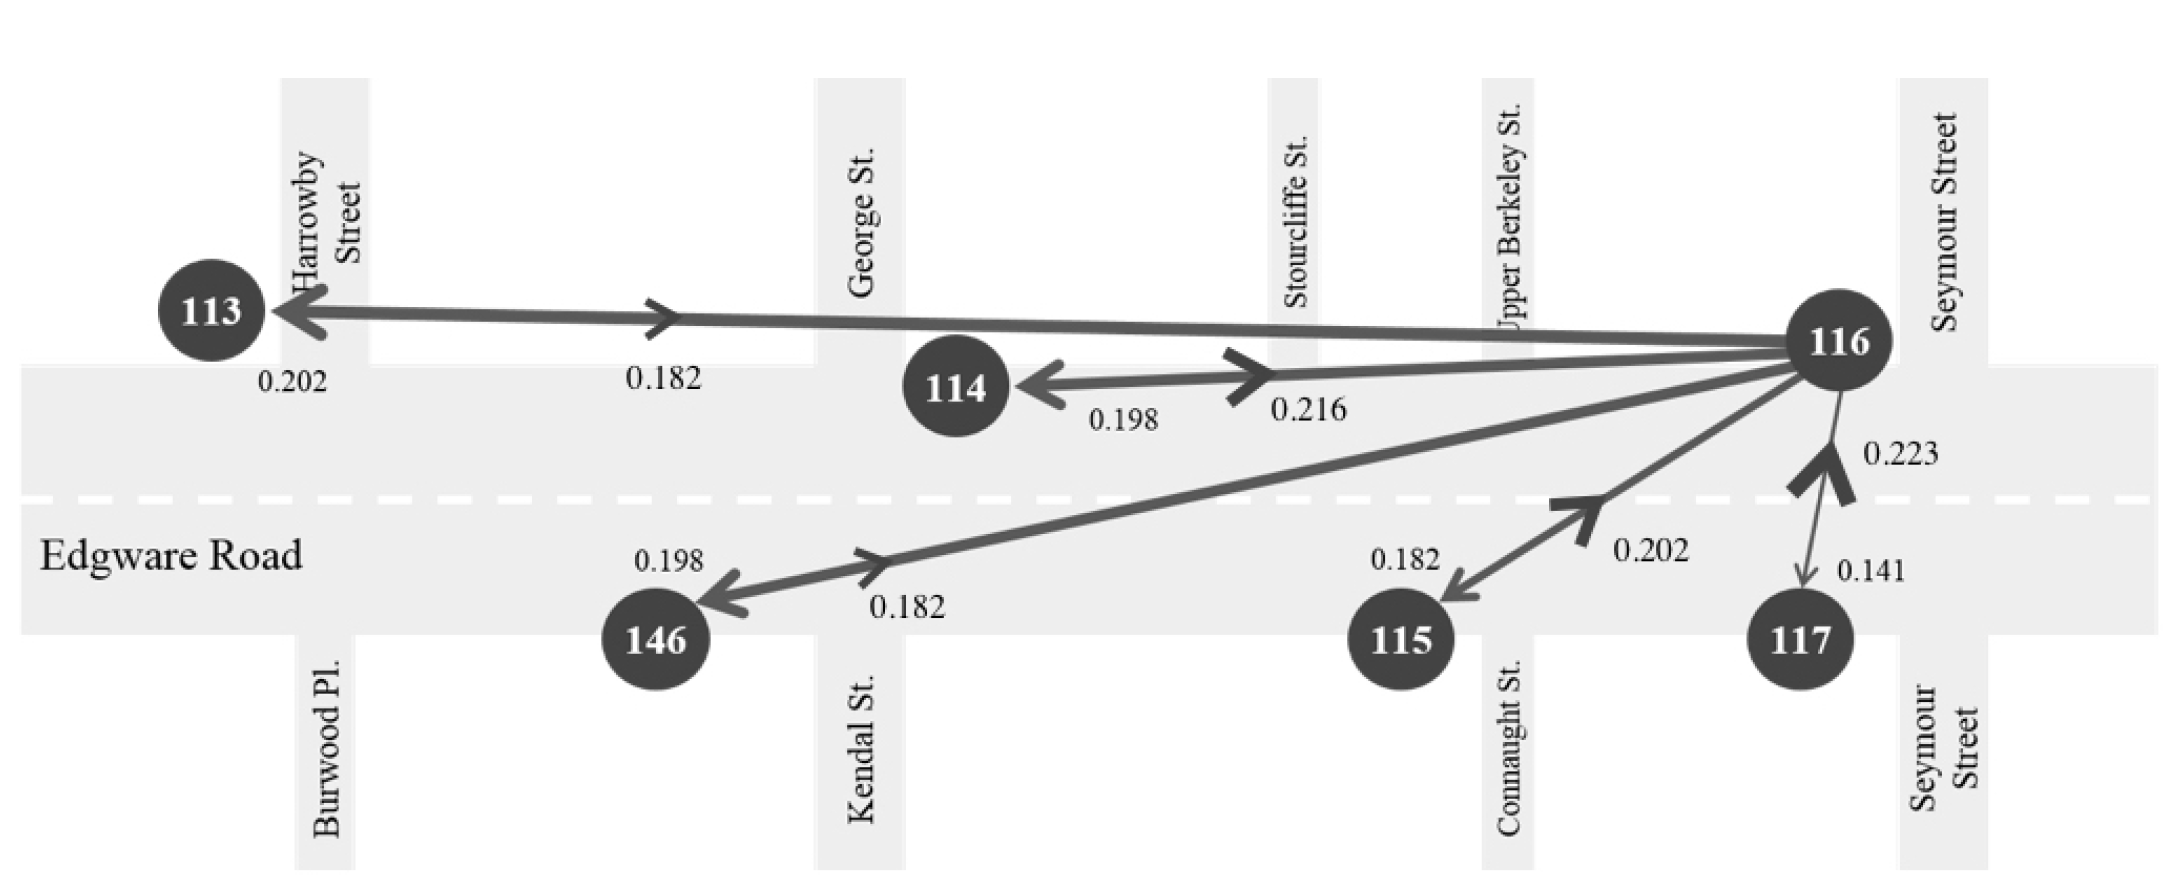
\includegraphics[trim={0 0 0 0},clip]{images/applications-transfer-entropy.png}
  \caption{Illustration of transfer entropies between set of locations along Edgware Road, London.}
  \label{figure:applications:transent}
\end{figure*}

Taking again Figure \ref{figure:applications:transent} as a reference, we measured the $TE$ between sensor 116 and the rest of the sensors.
The walking time is not constant and each sensor has counts at all times $i$, $j$.
There are people passing by these sensors that came from locations outside the network.
The numbers at each line represent the $TE$ measured between each pair of sensor locations.
The largest $TE$ value found was between 117 and 115.
The asymmetry of the TE is clear here, as the value in the opposite direction (115 to 117) is considerably lower.
Another interesting value is the pair 116-117, where TE(116,117) << TE(117,116).
This demonstrates that in this four-way crossing, the predominant direction of flow is from Location 117 to Location 116 (from the bottom of the figure upwards, or from west to east in reality). 
These results suggest that, in general, there is a larger flow of people from the west side to the east side of Edgware Road, and a larger flow of people from south to north of it. 
The results are consistent with our intuition that there is a larger flow of people from south to north along this road towards Edgware Road underground station.

There is still a series of uncertainties yet to be addressed by this model, such as the decay of probabilities with distance and the number of interventions of opportunity encountered by people while walking from one sensor to another.
However, this first initial set of results is encouraging in measuring flow between spatial points without actually tracking these users.
